\documentclass[12pt,journal]{IEEEtran}

\usepackage[utf8]{inputenc}
\usepackage[T1]{fontenc}
\usepackage[indonesian]{babel}
\usepackage{mathptmx}
\usepackage[expansion=false]{microtype}
\usepackage{amsmath,amssymb}
\usepackage{graphicx}
\usepackage{booktabs}
\usepackage{array}
\usepackage{cite}
\usepackage{placeins}
\usepackage[caption=false,font=footnotesize]{subfig}
\usepackage{tikz}
\usetikzlibrary{shapes.geometric, arrows.meta, positioning}

\AtBeginDocument{%
  \renewcommand{\figurename}{Gambar}%
  \renewcommand{\tablename}{Tabel}%
  \renewcommand{\refname}{Daftar Pustaka}%
  \renewcommand{\abstractname}{Abstrak}%
  \renewcommand{\IEEEkeywordsname}{Kata Kunci}%
}

\setlength{\parskip}{0pt plus 1pt}
\setlength{\emergencystretch}{2em}
\raggedbottom

\begin{document}

\title{Steganografi Citra Batik Nusantara Menggunakan Metode Pixel-Value Differencing dan Fungsi Modulus (PVDM) dengan Tabel Rentang Kuantisasi Asimetris Berbasis Human Visual System pada Ruang Warna RGB}

\author{Nama Penulis%
\thanks{Naskah diajukan November 2026. Penulis berasal dari Program Studi Informatika / Ilmu Komputer (Afiliasi Penulis).}}

\maketitle

\begin{abstract}
Steganografi domain spasial berbasis \textit{Pixel-Value Differencing and Modulus Function} (PVDM) mampu menekan distorsi citra, tetapi formulasi \textit{grayscale} klasik dan perluasan RGB berbasis \textit{Pixel Indicator} masih mengalami pemborosan kapasitas serta memperlakukan seluruh kanal warna secara seragam tanpa mempertimbangkan persepsi visual manusia. Penelitian ini mengusulkan metode PVDM RGB penuh (tiga kanal aktif simultan) dengan tabel rentang kuantisasi asimetris berbasis \textit{Human Visual System} (HVS) dan bobot luminansi ITU-R BT.601-7: kanal Green diproteksi dengan tabel 7-level (maksimal 2 bit per pasangan piksel pada area halus), kanal Red menggunakan tabel standar 6-level, dan kanal Blue diekspansi menjadi 5-level (minimal 4 bit pada area halus). Metode usulan (Skema 3) dievaluasi secara terkontrol (\textit{Batik vs.\ Batik}) terhadap re-implementasi \textit{Modified Pixel Indicator} Awate dan Patil (Skema 1) serta PVDM RGB Simetris 6-level (Skema 2) pada 45 citra Batik Nusantara ($512 \times 512$, 24-bit PNG \textit{lossless}) yang mencakup motif Parang, Kawung, dan Megamendung. Hasil eksperimen menunjukkan Skema 3 mencapai kapasitas rata-rata 168.175 byte (5,13 bpp) pada Parang, 171.475 byte (5,23 bpp) pada Kawung, dan 162.182 byte (4,95 bpp) pada Megamendung, meningkat +519,29\% hingga +566,33\% dibanding Skema 1 dan +1,34\% hingga +2,09\% dibanding Skema 2. Proteksi HVS terbukti konsisten: $\text{PSNR}_G$ selalu tertinggi di seluruh motif dan ukuran pesan (40,43--53,09 dB), $\text{SSIM}_Y$ mengungguli Skema 2 hingga kapasitas penuh (0,9969--0,9981), $\text{SSIM}_{\text{RGB}} > 0{,}99$ terjaga hingga 100 KB, serta ekstraksi buta mencapai 100\% \textit{lossless} ($\text{BER} = 0{,}0\%$) dengan korelasi tekstur-kapasitas sangat kuat ($r = 0{,}9574$).
\end{abstract}

\begin{IEEEkeywords}
Steganografi citra, pixel-value differencing and modulus function (PVDM), human visual system (HVS), tabel rentang asimetris, ruang warna RGB, Batik Nusantara.
\end{IEEEkeywords}

\section{Pendahuluan}

\IEEEPARstart{S}{teganografi} citra digital domain spasial bertujuan menyembunyikan pesan rahasia di dalam citra penampung (\textit{cover image}) tanpa menimbulkan anomali visual maupun statistik yang mencolok. Tantangan utama dalam pengolahan citra digital murni adalah menjaga keseimbangan antara kapasitas penyisipan (\textit{payload}) dan kualitas visual (\textit{imperceptibility}). Metode \textit{Pixel-Value Differencing and Modulus Function} (PVDM) yang diperkenalkan oleh Wang dkk.~\cite{wang2008high} menjawab tantangan tersebut dengan menyesuaikan jumlah bit pesan berdasarkan tingkat ketajaman tepi lokal serta meminimalkan pergeseran piksel melalui operasi sisa bagi (\textit{modulus}).

Meskipun efektif, masih terdapat dua celah penelitian (\textit{research gap}) penting pada literatur PVDM. Pertama, Wang dkk.~\cite{wang2008high} merumuskan PVDM hanya untuk citra \textit{grayscale} 8-bit satu kanal sehingga dua pertiga kapasitas warna pada citra RGB 24-bit tidak termanfaatkan. Kedua, perluasan RGB oleh Awate dan Patil~\cite{awate2016high} menggunakan skema \textit{Modified Pixel Indicator} (PI) yang mengorbankan seluruh kanal Red sebagai indikator 2 bit \textit{Least Significant Bit} (LSB). Ketika 2 bit LSB kanal Red bernilai \texttt{00} atau \texttt{11} (probabilitas 50\%), pasangan piksel dilewati; ketika \texttt{01} atau \texttt{10}, penyisipan hanya dilakukan pada salah satu kanal (Green atau Blue). Akibatnya, lebih dari 83\% potensi kapasitas RGB terbuang, dan tabel rentang 6-level tetap diterapkan seragam pada kanal Green maupun Blue tanpa memperhitungkan kepekaan \textit{Human Visual System} (HVS).

Untuk mengatasi permasalahan tersebut, penelitian ini mengusulkan skema PVDM RGB penuh yang mengaktifkan ketiga kanal warna secara simultan dengan tabel rentang kuantisasi asimetris berbasis HVS (Green protektif, Red standar, dan Blue ekspansif). Guna menjamin perbandingan yang adil (\textit{apple-to-apple}), metode Awate dan Patil (Skema 1) serta PVDM RGB Simetris 6-level (Skema 2) direplikasi secara langsung dan diuji pada dataset Batik Nusantara yang identik dengan metode usulan (Skema 3) sebagai variabel kontrol.

Citra Batik Nusantara ($512 \times 512$, 24-bit RGB) dipilih sebagai objek uji berdasarkan empat alasan teknis:
\begin{enumerate}
    \item \textit{Dualitas Frekuensi Spasial:} Motif Batik memadukan area gradasi halus (Megamendung) dan ornamen geometris rapat berfrekuensi tinggi (\textit{isen-isen} pada Parang dan Kawung).
    \item \textit{Uji Tekanan Alami FOBP:} Kontras tajam antara garis putih bekas lilin malam dan warna dasar gelap/\textit{sogan} memicu kasus \textit{Falling-Off-Boundary Problem} (FOBP) secara intensif.
    \item \textit{Ketimpangan Distribusi Warna (Chroma Skewness):} Palet Batik klasik didominasi warna gelap dengan intensitas kanal Blue rendah mendekati 0, menjadikannya medan uji yang ketat bagi stabilitas tabel ekspansif kanal Blue.
    \item \textit{Relevansi Domain:} Penyisipan tanpa distorsi visual mendukung perlindungan metadata kepemilikan dan hak cipta warisan budaya Batik Nusantara.
\end{enumerate}

Kontribusi utama penelitian ini meliputi: (1) perancangan tabel rentang kuantisasi asimetris berbasis HVS yang diturunkan dari bobot luminansi ITU-R BT.601-7 dan fisiologi retina; (2) evaluasi terkontrol \textit{Batik vs.\ Batik} terhadap dua metode pembanding yang membuktikan kenaikan kapasitas +519,29\% hingga +566,33\% dengan $\text{BER} = 0{,}0\%$; serta (3) analisis korelasi kuantitatif antara kerapatan tepi tekstur Batik, kapasitas penyisipan, dan frekuensi pemicuan FOBP.

\section{Tinjauan Pustaka dan Landasan Teori}

\subsection{Metode PVDM (Wang dkk., 2008)}
Wang dkk.~\cite{wang2008high} membagi citra menjadi pasangan piksel horizontal berurutan yang tidak tumpang tindih $(P_{(i,x)}, P_{(i,y)})$. Selisih mutlak $d_i = |P_{(i,x)} - P_{(i,y)}|$ dipetakan ke tabel rentang 6-level $R_j = [l_j, u_j]$ dengan lebar pangkat dua $w_j = u_j - l_j + 1$, yang menentukan kapasitas bit $t = \lfloor \log_2(w_j) \rfloor$. Alih-alih mengubah $d_i$ secara langsung, PVDM menyisipkan nilai desimal pesan $b$ ke dalam sisa bagi $\text{FREM}_i = (P_{(i,x)} + P_{(i,y)}) \bmod 2^t$ menggunakan aturan pergeseran optimal 8 kasus dan revisi FOBP 3 kasus.

\subsection{Steganografi RGB Berbasis Modified Pixel Indicator (Awate dan Patil, 2016)}
Awate dan Patil~\cite{awate2016high} memperluas PVDM ke ruang warna RGB dengan membaca 2 bit LSB kanal Red pada piksel pertama setiap pasangan: \texttt{00} dan \texttt{11} melewatkan pasangan piksel, \texttt{01} menyisipkan data hanya pada Green, dan \texttt{10} hanya pada Blue. Karena kanal Red tidak pernah diubah ($\text{MSE}_R = 0$), rata-rata pemanfaatan kanal hanya $(0{,}25 \times 1) + (0{,}25 \times 1) = 0{,}5$ dari 3 kanal (16,67\% aktif, 83,33\% terbuang), sementara Green dan Blue tetap memakai tabel 6-level yang sama.

\subsection{HVS, Standar ITU-R BT.601-7, dan Keseimbangan Luminansi}
Berdasarkan standar internasional ITU-R BT.601-7~\cite{itur2011bt601}, sinyal luminansi $Y$ yang merepresentasikan persepsi kecerahan dan ketajaman tepi mata manusia dikonstruksi dari kanal RGB melalui persamaan:
\begin{equation}
Y = 0{,}299R + 0{,}587G + 0{,}114B
\label{eq:bt601}
\end{equation}
Pada kuantisasi 8-bit, bobot masing-masing kanal adalah $150/256$ (58,7\%) untuk Green, $77/256$ (29,9\%) untuk Red, dan $29/256$ (11,4\%) untuk Blue. Pemetaan anatomi retina manusia hidup oleh Roorda dan Williams~\cite{roorda1999arrangement} memperkuat fakta ini: sel kerucut penerima gelombang pendek (S-cones / Biru) hanya berjumlah kurang dari 6--10\% dan absen di pusat penglihatan tajam (\textit{foveola}), sedangkan M-cones (Hijau) dan L-cones (Merah) mendominasi lebih dari 90\% dengan puncak sensitivitas fotopik di spektrum hijau ($\approx 555$~nm).

Mengacu pada prinsip \textit{Just Noticeable Difference} (JND), pembatasan pergeseran maksimal pada area halus sebesar $\pm 1$ untuk Green ($t=2$), $\pm 2$ untuk Red ($t=3$), dan $\pm 4$ untuk Blue ($t=4$) menghasilkan kontribusi perubahan luminansi yang hampir seimbang antar kanal ($\Delta Y_G = 0{,}587$, $\Delta Y_R = 0{,}598$, $\Delta Y_B = 0{,}456$) dengan total $\Delta Y = 1{,}641$ (0,6\% dari rentang 0--255), sehingga tidak memicu pergeseran rona warna (\textit{no hue shift}). Pada area tepi tajam, pergeseran piksel yang lebih besar tertutup secara alami oleh efek \textit{spatial contrast masking}. Posisi penelitian ini dibandingkan literatur utama dirangkum pada Tabel~\ref{tab:research_gap}.

\begin{table*}[t]
\centering
\caption{Posisi Riset dan Perbandingan Celah Penelitian}
\label{tab:research_gap}
\footnotesize
\setlength{\tabcolsep}{5pt}
\resizebox{\textwidth}{!}{%
\begin{tabular}{@{}llll@{}}
\toprule
Aspek Perbandingan & Wang dkk. (2008)~\cite{wang2008high} & Awate dan Patil (2016)~\cite{awate2016high} & Metode Usulan (Skema 3) \\
\midrule
Ruang Warna & Grayscale (1 kanal, 8-bit) & RGB (3 kanal, 24-bit, PI) & RGB Penuh (3 kanal aktif, 24-bit) \\
Pemanfaatan Kanal & 1 kanal & Red jadi indikator 2-LSB ($>$83\% terbuang) & Penyisipan simultan di R, G, dan B \\
Desain Tabel Rentang & 1 tabel statis 6-level & 1 tabel statis 6-level untuk G dan B & 3 tabel asimetris HVS (G: 7, R: 6, B: 5 level) \\
Analisis Citra & Citra standar (Lena, Baboon) & Citra standar tanpa analisis tekstur & Tekstur Batik Nusantara, distribusi $d_i$, laju FOBP \\
\bottomrule
\end{tabular}%
}
\end{table*}

\FloatBarrier

\section{Metodologi yang Diusulkan}

\subsection{Arsitektur Sistem}
Gambar~\ref{fig:architecture} menampilkan alur penyisipan (\textit{embedding}) dan ekstraksi buta (\textit{blind extraction}). Citra penampung RGB 24-bit ($512 \times 512 \times 3$) dipisah menjadi kanal Red, Green, dan Blue. Sebelum dikonversi ke deretan bit (\textit{MSB-first}), pesan rahasia diawali \textit{header} panjang pesan 32-bit (\texttt{uint32} \textit{big-endian}) agar proses ekstraksi dapat berhenti tepat di akhir pesan tanpa memerlukan citra asli. Ketiga kanal diproses menggunakan tabel rentang asimetris HVS masing-masing, lalu digabungkan kembali menjadi citra stego berformat PNG \textit{lossless}.

\begin{figure*}[t]
\centering
\resizebox{\textwidth}{!}{%
\begin{tikzpicture}[
    node distance=0.55cm and 0.65cm,
    box/.style={rectangle, draw, rounded corners=2pt, minimum height=0.85cm, minimum width=2.2cm, align=center, font=\footnotesize},
    arrow/.style={-{Stealth[length=2mm]}, thick}
]
\node[box] (cover) {Citra Cover RGB\\($512\times 512\times 3$)};
\node[box, right=of cover] (split) {Pemisahan Kanal\\(R, G, B)};
\node[box, right=of split] (hdr) {Header 32-bit\\+ Aliran Bit};
\node[box, right=of hdr] (asym) {PVDM Asimetris\\(G:7, R:6, B:5)};
\node[box, right=of asym] (fobp) {Step 4 FOBP\\+ Sub-range Guard};
\node[box, right=of fobp] (stego) {Citra Stego\\(PNG Lossless)};

\draw[arrow] (cover) -- (split);
\draw[arrow] (split) -- (asym);
\draw[arrow] (hdr) -- (asym);
\draw[arrow] (asym) -- (fobp);
\draw[arrow] (fobp) -- (stego);

\node[box, below=1.1cm of cover] (stego2) {Citra Stego RGB\\(PNG Lossless)};
\node[box, right=of stego2] (split2) {Pemisahan Kanal\\(R, G, B)};
\node[box, right=of split2] (diff2) {Hitung $d_i^*$\\Cari Nilai $t_c$};
\node[box, right=of diff2] (mod2) {Ekstrak $b=$\\$(P_x^*+P_y^*)\bmod 2^t$};
\node[box, right=of mod2] (unp) {Baca Header\\Panjang 32-bit};
\node[box, right=of unp] (rec) {Pesan Pulih\\($\text{BER}=0\%$)};

\draw[arrow] (stego2) -- (split2);
\draw[arrow] (split2) -- (diff2);
\draw[arrow] (diff2) -- (mod2);
\draw[arrow] (mod2) -- (unp);
\draw[arrow] (unp) -- (rec);
\end{tikzpicture}%
}
\caption{Diagram alir arsitektur sistem PVDM RGB asimetris berbasis HVS untuk proses penyisipan (atas) dan ekstraksi buta (bawah).}
\label{fig:architecture}
\end{figure*}

\subsection{Desain Tabel Rentang Kuantisasi Asimetris HVS}
Untuk setiap kanal $c \in \{R, G, B\}$, rentang selisih $[0, 255]$ dibagi menjadi sub-rentang $R_j = [l_j, u_j]$ dengan lebar $w_j = u_j - l_j + 1$ berupa pangkat dua dan kapasitas $t = \lfloor \log_2(w_j) \rfloor$, sebagaimana ditunjukkan pada Tabel~\ref{tab:range_tables}. Pemecahan area halus $[0, 7]$ menjadi $[0, 3]$ dan $[4, 7]$ ($w=4, t=2$) pada kanal Green menjaga pergeseran maksimal $\pm 1$, sedangkan penggabungan $[0, 15]$ ($w=16, t=4$) pada kanal Blue meningkatkan kapasitas dasar di area halus.

\begin{table*}[t]
\centering
\caption{Tabel Rentang Kuantisasi Asimetris Berbasis HVS ($R_j = [l_j, u_j]$)}
\label{tab:range_tables}
\footnotesize
\begin{tabular}{@{}llll@{}}
\toprule
Level & Green (7-Level, Protektif) & Red (6-Level, Standar) & Blue (5-Level, Ekspansif) \\
\midrule
$R_1$ & $[0, 3], w=4, t=2$     & $[0, 7], w=8, t=3$     & $[0, 15], w=16, t=4$ \\
$R_2$ & $[4, 7], w=4, t=2$     & $[8, 15], w=8, t=3$    & $[16, 31], w=16, t=4$ \\
$R_3$ & $[8, 15], w=8, t=3$    & $[16, 31], w=16, t=4$  & $[32, 63], w=32, t=5$ \\
$R_4$ & $[16, 31], w=16, t=4$  & $[32, 63], w=32, t=5$  & $[64, 127], w=64, t=6$ \\
$R_5$ & $[32, 63], w=32, t=5$  & $[64, 127], w=64, t=6$ & $[128, 255], w=128, t=7$ \\
$R_6$ & $[64, 127], w=64, t=6$ & $[128, 255], w=128, t=7$ & --- \\
$R_7$ & $[128, 255], w=128, t=7$ & ---                  & --- \\
\bottomrule
\end{tabular}
\end{table*}

\subsection{Algoritma Penyisipan (Step 1--4) dan Sub-Range Guard}
Pada setiap kanal $c$, citra dibagi menjadi pasangan piksel horizontal $(P_{(i,x)}, P_{(i,y)})$ dengan indeks $i = 1, \dots, MN/2$, kemudian diproses sebagai berikut:
\begin{enumerate}
    \item \textit{Step 1 (Selisih dan Kapasitas):} Hitung $d_i = |P_{(i,x)} - P_{(i,y)}|$, petakan ke Tabel~\ref{tab:range_tables} untuk memperoleh $w_j$ dan $t = \lfloor \log_2(w_j) \rfloor$, lalu ambil $t$ bit dari aliran pesan rahasia menjadi nilai desimal $b$.
    \item \textit{Step 2 (Sisa Bagi):} Hitung nilai sisa bagi modular:
    \begin{equation}
    \text{FREM}_i = (P_{(i,x)} + P_{(i,y)}) \bmod 2^t
    \label{eq:frem}
    \end{equation}
    \item \textit{Step 3 (Pergeseran Optimal 8 Kasus):} Hitung jarak $m = |\text{FREM}_i - b|$ dan komplemennya $m_1 = 2^t - m$. Ubah $(P_{(i,x)}, P_{(i,y)})$ menjadi $(P'_{(i,x)}, P'_{(i,y)})$ sesuai Tabel~\ref{tab:step3_4}. Pembulatan bersilang $\lceil \cdot \rceil$ dan $\lfloor \cdot \rfloor$ berdasarkan urutan $P_{(i,x)} \ge P_{(i,y)}$ mempertahankan selisih baru $d' = |P'_{(i,x)} - P'_{(i,y)}|$ tetap rapat sehingga meminimalkan MSE dan mencegah perpindahan sub-rentang.
    \item \textit{Step 4 (Revisi FOBP 3 Kasus dan Sub-Range Guard):} Apabila $P'_{(i,x)}$ atau $P'_{(i,y)}$ keluar dari batas $[0, 255]$, terapkan revisi FOBP pada Tabel~\ref{tab:step3_4}. Jika $d'$ melompat keluar dari $[l_j, u_j]$, mekanisme \textit{Sub-range Guard} mencari pasangan sah terdekat di dalam $[l_j, u_j]$ dengan $(P''_{(i,x)} + P''_{(i,y)}) \bmod 2^t = b$ ber-MSE minimum untuk menjamin ekstraksi 100\% \textit{lossless}.
\end{enumerate}

\begin{table*}[t]
\centering
\caption{Ringkasan 8 Kasus Pergeseran Optimal (Step 3) dan 3 Kasus Penanganan FOBP (Step 4)}
\label{tab:step3_4}
\footnotesize
\setlength{\tabcolsep}{4pt}
\resizebox{\textwidth}{!}{%
\begin{tabular}{@{}llll@{}}
\toprule
Tahap & Kasus & Kondisi & Modifikasi Piksel $(P'_{(i,x)}, P'_{(i,y)})$ atau $(P''_{(i,x)}, P''_{(i,y)})$ \\
\midrule
Step 3 & Kasus 1 & $\text{FREM}_i > b,\; m \le 2^{t-1},\; P_{(i,x)} \ge P_{(i,y)}$ & $(P_{(i,x)} - \lceil m/2 \rceil,\; P_{(i,y)} - \lfloor m/2 \rfloor)$ \\
       & Kasus 2 & $\text{FREM}_i > b,\; m \le 2^{t-1},\; P_{(i,x)} < P_{(i,y)}$   & $(P_{(i,x)} - \lfloor m/2 \rfloor,\; P_{(i,y)} - \lceil m/2 \rceil)$ \\
       & Kasus 3 & $\text{FREM}_i > b,\; m > 2^{t-1},\; P_{(i,x)} \ge P_{(i,y)}$   & $(P_{(i,x)} + \lfloor m_1/2 \rfloor,\; P_{(i,y)} + \lceil m_1/2 \rceil)$ \\
       & Kasus 4 & $\text{FREM}_i > b,\; m > 2^{t-1},\; P_{(i,x)} < P_{(i,y)}$     & $(P_{(i,x)} + \lceil m_1/2 \rceil,\; P_{(i,y)} + \lfloor m_1/2 \rfloor)$ \\
       & Kasus 5 & $\text{FREM}_i \le b,\; m \le 2^{t-1},\; P_{(i,x)} \ge P_{(i,y)}$ & $(P_{(i,x)} + \lfloor m/2 \rfloor,\; P_{(i,y)} + \lceil m/2 \rceil)$ \\
       & Kasus 6 & $\text{FREM}_i \le b,\; m \le 2^{t-1},\; P_{(i,x)} < P_{(i,y)}$   & $(P_{(i,x)} + \lceil m/2 \rceil,\; P_{(i,y)} + \lfloor m/2 \rfloor)$ \\
       & Kasus 7 & $\text{FREM}_i \le b,\; m > 2^{t-1},\; P_{(i,x)} \ge P_{(i,y)}$   & $(P_{(i,x)} - \lceil m_1/2 \rceil,\; P_{(i,y)} - \lfloor m_1/2 \rfloor)$ \\
       & Kasus 8 & $\text{FREM}_i \le b,\; m > 2^{t-1},\; P_{(i,x)} < P_{(i,y)}$     & $(P_{(i,x)} - \lfloor m_1/2 \rfloor,\; P_{(i,y)} - \lceil m_1/2 \rceil)$ \\
\midrule
Step 4 & FOBP 1 & $d_i \le 128$ dan ($P'_{(i,x)} < 0$ atau $P'_{(i,y)} < 0$)     & $(P'_{(i,x)} + 2^{t-1},\; P'_{(i,y)} + 2^{t-1})$ \\
       & FOBP 2 & $d_i \le 128$ dan ($P'_{(i,x)} > 255$ atau $P'_{(i,y)} > 255$) & $(P'_{(i,x)} - 2^{t-1},\; P'_{(i,y)} - 2^{t-1})$ \\
       & FOBP 3 & $d_i > 128$ dan terjadi \textit{overflow}/\textit{underflow} & Kunci piksel ke $0$ atau $255$, geser sisa ke pasangannya \\
\bottomrule
\end{tabular}%
}
\end{table*}

\subsection{Algoritma Ekstraksi Buta}
Dari citra stego RGB, setiap kanal dibagi menjadi pasangan piksel $(P^*_{(i,x)}, P^*_{(i,y)})$. Penerima menghitung $d^*_i = |P^*_{(i,x)} - P^*_{(i,y)}|$, menentukan $t$ dari Tabel~\ref{tab:range_tables}, lalu mengekstrak nilai desimal pesan:
\begin{equation}
b = (P^*_{(i,x)} + P^*_{(i,y)}) \bmod 2^t
\label{eq:extract}
\end{equation}
Setiap nilai $b$ dikonversi kembali menjadi biner sepanjang $t$ bit; 32 bit pertama dibaca sebagai panjang byte pesan asli untuk menghentikan ekstraksi secara tepat.

\subsection{Desain Eksperimen Terkontrol dan Metrik Evaluasi}
Dataset uji terdiri atas 45 citra Batik Nusantara ($512 \times 512$, 24-bit PNG \textit{lossless}), masing-masing 15 citra untuk motif Parang, Kawung, dan Megamendung (Gambar~\ref{fig:dataset}). Ketiga skema diuji menggunakan pesan byte acak deterministik (\texttt{seed=2026}) pada empat ukuran \textit{payload}: 10~KB, 50~KB, 100~KB, dan Kapasitas Penuh (\textit{Full}).

\begin{figure}[t]
\centering
\subfloat[Parang]{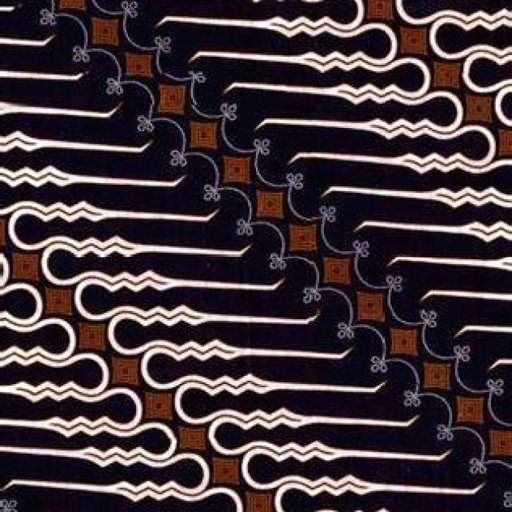
\includegraphics[width=0.31\linewidth]{figures/parang_01.png}}\hfill
\subfloat[Kawung]{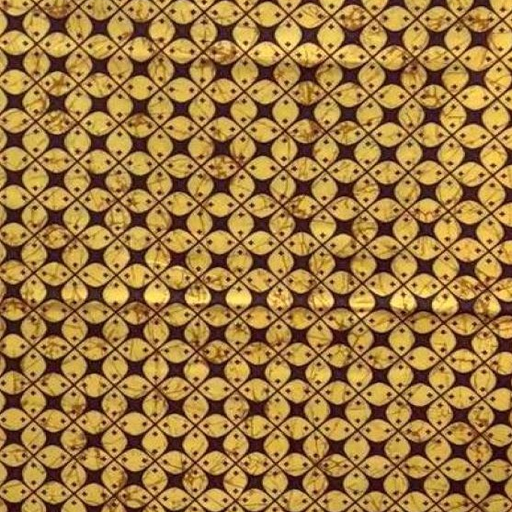
\includegraphics[width=0.31\linewidth]{figures/kawung_01.png}}\hfill
\subfloat[Megamendung]{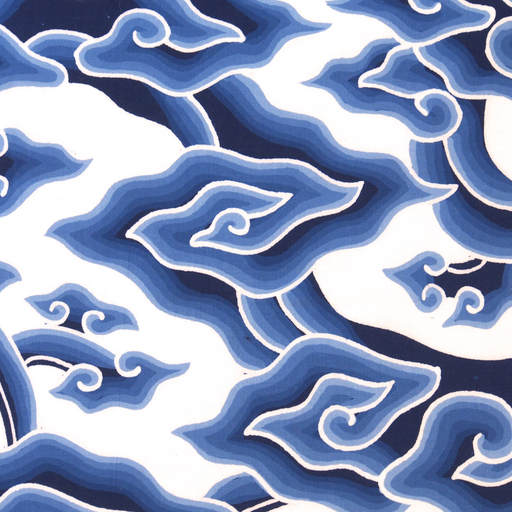
\includegraphics[width=0.31\linewidth]{figures/megamendung_01.png}}
\caption{Sampel citra penampung Batik Nusantara berukuran $512 \times 512$ piksel (24-bit RGB) untuk motif Parang, Kawung, dan Megamendung.}
\label{fig:dataset}
\end{figure}

Kapasitas total, laju penyisipan ($\text{bpp}$), MSE, PSNR, SSIM~\cite{wang2004image}, BER, laju FOBP, dan korelasi Pearson $r$ dihitung melalui persamaan berikut:
\begin{equation}
\text{Cap}_{\text{Total}} = \sum_{i=1}^{MN/2} \left(t_{R,i} + t_{G,i} + t_{B,i}\right)
\label{eq:cap}
\end{equation}
\begin{equation}
\text{bpp} = \frac{\text{Cap}_{\text{Total}}}{H \times W}
\label{eq:bpp}
\end{equation}
\begin{align}
\text{MSE}_c &= \frac{1}{HW} \sum_{x=0}^{H-1} \sum_{y=0}^{W-1} \left(I_c(x,y) - S_c(x,y)\right)^2 \label{eq:mse_c}\\
\text{MSE}_{\text{RGB}} &= \frac{\text{MSE}_R + \text{MSE}_G + \text{MSE}_B}{3} \label{eq:mse}
\end{align}
\begin{equation}
\text{PSNR}_{\text{RGB}} = 10 \log_{10}\left(\frac{255^2}{\text{MSE}_{\text{RGB}}}\right)\text{ dB}
\label{eq:psnr}
\end{equation}
\begin{equation}
\text{SSIM}(x,y) = \frac{(2\mu_x\mu_y + C_1)(2\sigma_{xy} + C_2)}{(\mu_x^2 + \mu_y^2 + C_1)(\sigma_x^2 + \sigma_y^2 + C_2)}
\label{eq:ssim}
\end{equation}
dengan $C_1 = (0{,}01 \times 255)^2$, $C_2 = (0{,}03 \times 255)^2$, serta jendela Gaussian $11 \times 11$ ($\sigma = 1{,}5$), dihitung per kanal ($\text{SSIM}_R$, $\text{SSIM}_G$, $\text{SSIM}_B$), rata-rata $\text{SSIM}_{\text{RGB}}$, dan kanal luminansi ITU-R BT.601 ($\text{SSIM}_Y$). Ketepatan ekstraksi, laju FOBP, dan korelasi Pearson didefinisikan sebagai:
\begin{align}
\text{BER} &= \frac{\text{Jumlah Bit Galat}}{\text{Total Bit Pesan}} \times 100\% \label{eq:ber}\\
\text{FOBP Rate} &= \frac{\text{Total FOBP}}{3 \times \text{Pasangan Terpakai}} \times 100\% \label{eq:ber_fobp}
\end{align}
\begin{equation}
r = \frac{\sum (x_i - \bar{x})(y_i - \bar{y})}{\sqrt{\sum (x_i - \bar{x})^2 \sum (y_i - \bar{y})^2}}
\label{eq:pearson}
\end{equation}

\FloatBarrier

\section{Hasil Eksperimen dan Pembahasan}

\subsection{Verifikasi Implementasi dan Uji Lossless}
Sebelum evaluasi penuh, mesin inti dan ketiga skema telah diverifikasi melalui 89 pengujian otomatis (\textit{89 passed, 0 failed}), mencakup replikasi presisi Tabel~2 dan Tabel~3 Wang dkk.~\cite{wang2008high}, pengujian individual seluruh 8 kasus Step~3, serta uji simpan-muat ulang PNG lintas motif. Pada seluruh 45 citra dan seluruh variasi ukuran pesan, ekstraksi buta menghasilkan $\text{BER} = 0{,}0\%$.

\subsection{Analisis Kapasitas Maksimum per Kanal (Batik vs.\ Batik)}
Tabel~\ref{tab:capacity} dan Gambar~\ref{fig:capacity} memperlihatkan perbandingan kapasitas maksimum pada 45 citra Batik. Skema~1 hanya mampu menampung rata-rata 24.339--27.623 byte (0,74--0,84 bpp) sehingga gagal menyisipkan pesan 50~KB dan 100~KB. Sebaliknya, Skema~3 mencapai rata-rata 168.175 byte (5,13 bpp) pada Parang, 171.475 byte (5,23 bpp) pada Kawung, dan 162.182 byte (4,95 bpp) pada Megamendung, unggul +519,29\% hingga +566,33\% terhadap Skema~1 dan +1,34\% hingga +2,09\% terhadap Skema~2. Alokasi kapasitas per kanal membuktikan desain asimetris bekerja optimal: Blue menampung porsi terbesar (66.959--68.116 byte), Red di posisi menengah (53.869--56.058 byte), dan Green paling dibatasi (41.354--47.682 byte).

\begin{table*}[t]
\centering
\caption{Analisis Kapasitas Maksimum per Kanal (Rata-Rata 15 Citra per Motif)}
\label{tab:capacity}
\footnotesize
\setlength{\tabcolsep}{4pt}
\resizebox{\textwidth}{!}{%
\begin{tabular}{@{}llrrrrrrrr@{}}
\toprule
Motif ($n=15$) & Skema & R (Byte) & G (Byte) & B (Byte) & Total (Byte) & Total (Bit) & BPP & Gain vs S1 & Gain vs S2 \\
\midrule
Parang      & Skema 1 (Awate \& Patil) & 0,00     & 13.667,40 & 13.488,53 & 27.156,33  & 217.254,00   & 0,8288 & 0,00\%    & $-$83,63\% \\
            & Skema 2 (Simetris)       & 55.296,73 & 55.433,07 & 55.150,93 & 165.881,60 & 1.327.055,80 & 5,0623 & +510,84\% & 0,00\% \\
            & Skema 3 (Usulan HVS)     & 55.296,73 & 44.761,40 & 68.116,27 & 168.175,33 & 1.345.405,93 & 5,1323 & +519,29\% & +1,38\% \\
\midrule
Kawung      & Skema 1 (Awate \& Patil) & 0,00     & 13.761,67 & 13.860,67 & 27.622,67  & 220.984,87   & 0,8430 & 0,00\%    & $-$83,55\% \\
            & Skema 2 (Simetris)       & 56.057,87 & 56.063,00 & 55.839,07 & 167.960,87 & 1.343.690,80 & 5,1258 & +508,05\% & 0,00\% \\
            & Skema 3 (Usulan HVS)     & 56.057,87 & 47.681,67 & 67.734,80 & 171.475,13 & 1.371.804,93 & 5,2330 & +520,78\% & +2,09\% \\
\midrule
Megamendung & Skema 1 (Awate \& Patil) & 0,00     & 12.160,33 & 12.178,60 & 24.339,47  & 194.718,80   & 0,7428 & 0,00\%    & $-$84,79\% \\
            & Skema 2 (Simetris)       & 53.868,53 & 53.372,00 & 52.792,93 & 160.034,33 & 1.280.278,00 & 4,8839 & +557,51\% & 0,00\% \\
            & Skema 3 (Usulan HVS)     & 53.868,53 & 41.353,67 & 66.958,53 & 162.181,73 & 1.297.457,27 & 4,9494 & +566,33\% & +1,34\% \\
\bottomrule
\end{tabular}%
}
\end{table*}

\begin{figure*}[t]
\centering
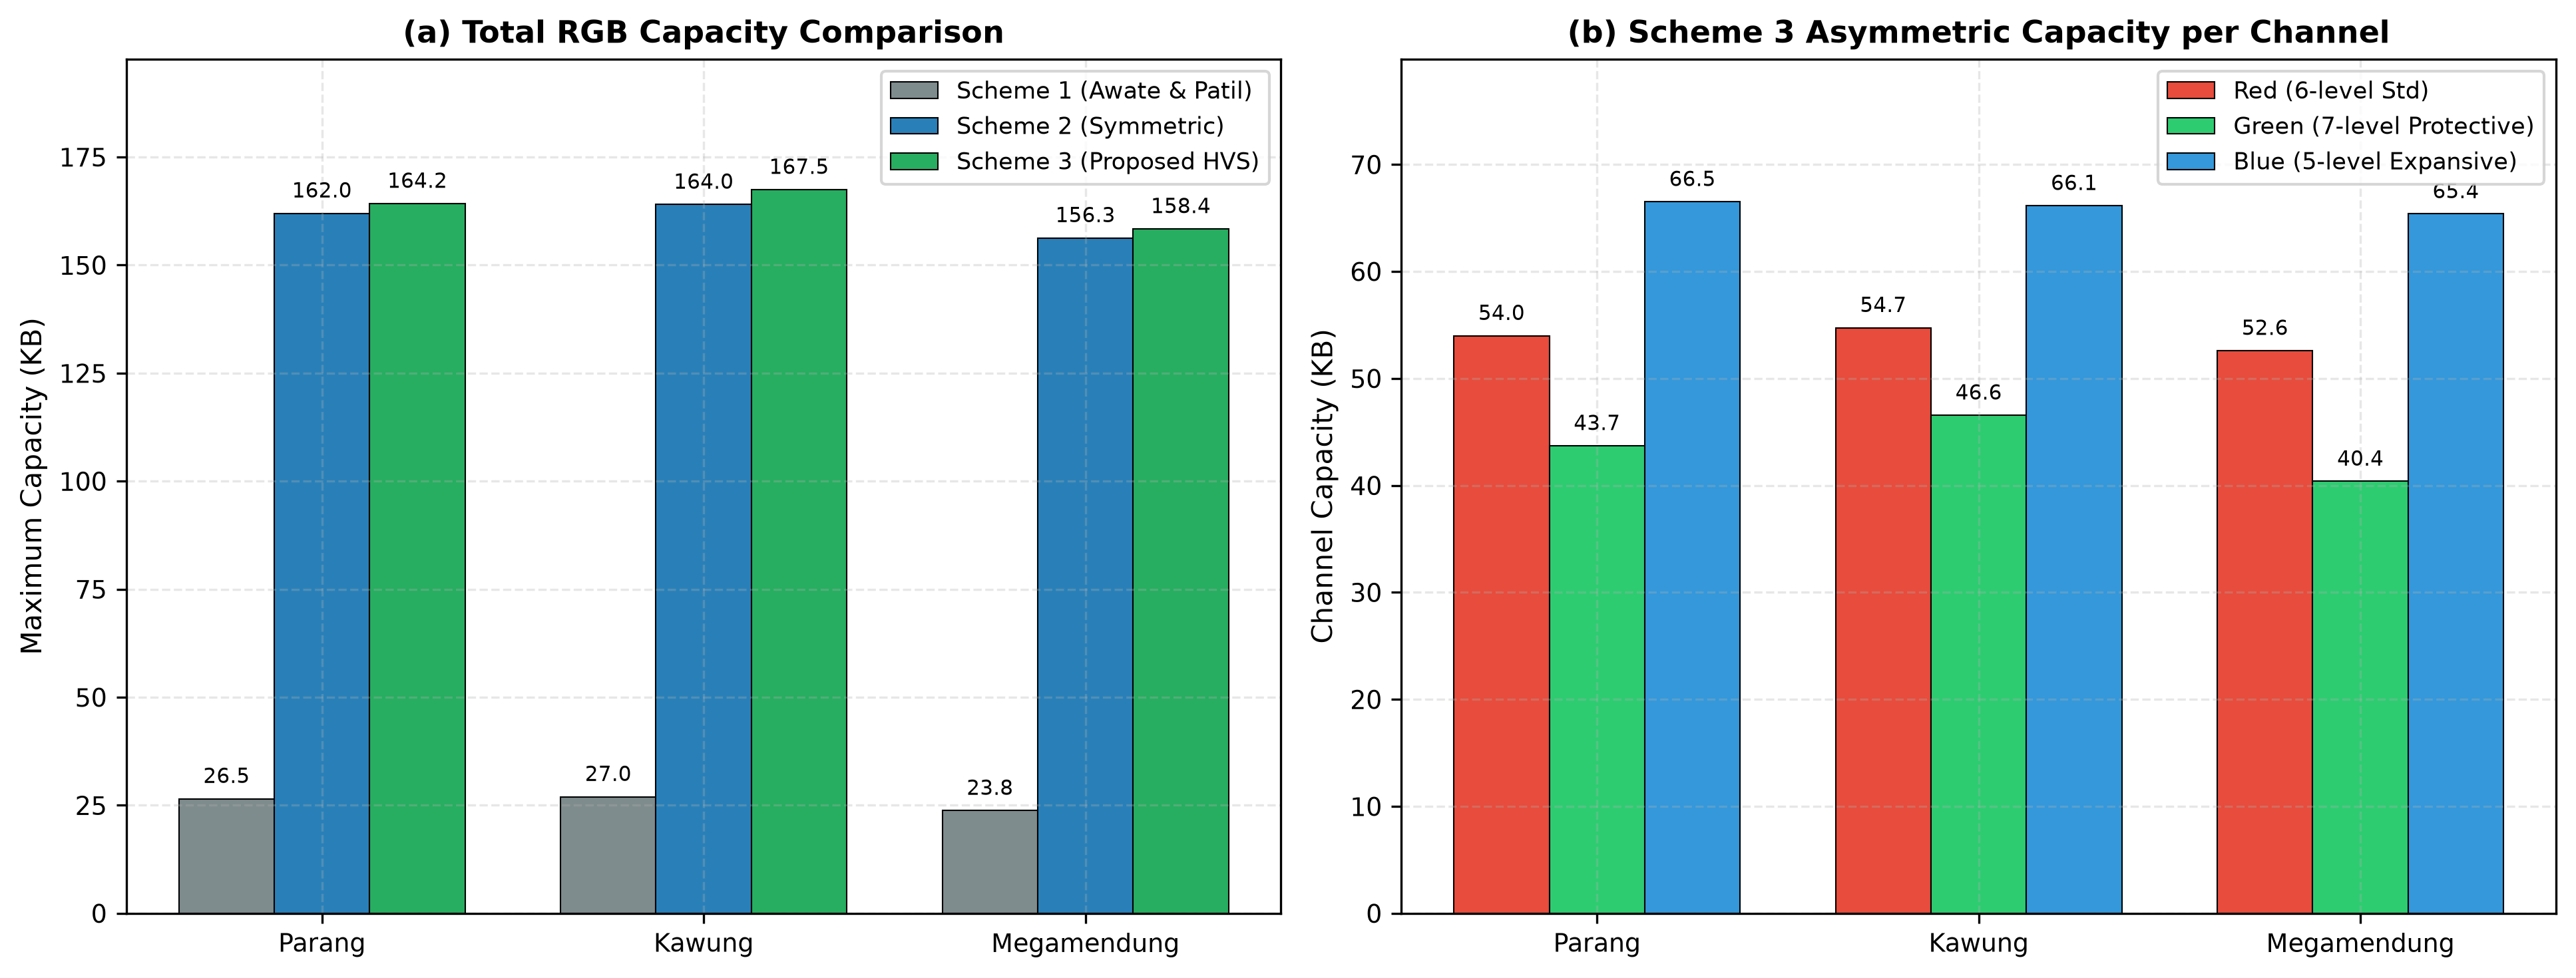
\includegraphics[width=0.92\linewidth]{figures/fig1_capacity_comparison.png}
\caption{Perbandingan kapasitas maksimum total RGB antar Skema 1--3 (a) dan alokasi kapasitas asimetris per kanal pada Skema 3 (b).}
\label{fig:capacity}
\end{figure*}

\subsection{Evaluasi Kualitas Citra Multimetrik dan Validasi HVS}
Tabel~\ref{tab:quality} dan Tabel~\ref{tab:per_channel_mse_ssim}, bersama Gambar~\ref{fig:psnr} dan Gambar~\ref{fig:ssim}, memvalidasi efektivitas proteksi kanal Green. Pada 100\% motif dan ukuran pesan pada Skema~3, kanal Green selalu mencatat nilai PSNR tertinggi (40,43--53,09~dB, lebih tinggi +0,59 hingga +1,06~dB dibanding $\text{PSNR}_G$ Skema~2), $\text{MSE}_G$ terendah (0,3613--8,2942), serta $\text{SSIM}_G$ tertinggi (0,9953--0,9998). Dampaknya, kualitas luminansi manusia ($\text{SSIM}_Y$) pada Skema~3 selalu mengungguli atau menyamai Skema~2 hingga kapasitas penuh (0,9969--0,9981 vs.\ 0,9955--0,9976), sedangkan $\text{SSIM}_{\text{RGB}}$ terjaga di atas 0,99 hingga \textit{payload} 100~KB (0,9902--0,9996).

\begin{table*}[t]
\centering
\caption{Evaluasi Kualitas Citra Multimetrik pada Variasi Payload (Rata-Rata 15 Citra per Motif)}
\label{tab:quality}
\scriptsize
\setlength{\tabcolsep}{3.5pt}
\resizebox{\textwidth}{!}{%
\begin{tabular}{@{}llrrrrrrrrrrr@{}}
\toprule
Motif & Skema & Ukuran & Payload (B) & $\text{MSE}_{\text{RGB}}$ & $\text{PSNR}_R$ & $\text{PSNR}_G$ & $\text{PSNR}_B$ & $\text{PSNR}_{\text{RGB}}$ & $\text{SSIM}_{\text{RGB}}$ & $\text{SSIM}_Y$ & BER & FOBP \\
\midrule
Parang      & Skema 1 & 10 KB  & 10.240  & 0,5317 & $\infty$ & 50,25 & 50,29 & 52,03 & 0,9994 & 0,9997 & 0,0\% & 412,80 \\
            & Skema 1 & Full   & 27.152  & 1,4867 & $\infty$ & 45,81 & 45,89 & 47,61 & 0,9984 & 0,9992 & 0,0\% & 1.197,27 \\
            & Skema 2 & 10 KB  & 10.240  & 0,5601 & 51,94 & 51,93 & 51,90 & 51,92 & 0,9995 & 0,9998 & 0,0\% & 506,13 \\
            & Skema 2 & 50 KB  & 51.200  & 2,6373 & 44,99 & 45,04 & 45,07 & 45,03 & 0,9970 & 0,9987 & 0,0\% & 2.480,93 \\
            & Skema 2 & 100 KB & 102.400 & 5,3015 & 41,92 & 41,96 & 42,02 & 41,97 & 0,9940 & 0,9974 & 0,0\% & 5.172,40 \\
            & Skema 2 & Full   & 165.878 & 9,0210 & 39,74 & 39,76 & 39,81 & 39,77 & 0,9903 & 0,9958 & 0,0\% & 8.846,80 \\
            & Skema 3 & 10 KB  & 10.240  & 0,6161 & 51,94 & 52,99 & 49,75 & 51,19 & 0,9992 & 0,9998 & 0,0\% & 547,73 \\
            & Skema 3 & 50 KB  & 51.200  & 2,9283 & 45,05 & 46,06 & 42,81 & 44,28 & 0,9952 & 0,9991 & 0,0\% & 2.692,67 \\
            & Skema 3 & 100 KB & 102.400 & 5,8635 & 41,99 & 42,95 & 39,78 & 41,23 & 0,9902 & 0,9982 & 0,0\% & 5.639,33 \\
            & Skema 3 & Full   & 168.171 & 10,0900 & 39,74 & 40,69 & 37,53 & 38,97 & 0,9839 & 0,9970 & 0,0\% & 9.822,07 \\
\midrule
Kawung      & Skema 1 & 10 KB  & 10.240  & 0,4056 & $\infty$ & 50,69 & 50,78 & 52,50 & 0,9997 & 0,9998 & 0,0\% & 264,67 \\
            & Skema 1 & Full   & 27.619  & 1,1125 & $\infty$ & 46,38 & 46,40 & 48,15 & 0,9992 & 0,9995 & 0,0\% & 716,47 \\
            & Skema 2 & 10 KB  & 10.240  & 0,4038 & 52,47 & 52,50 & 52,58 & 52,51 & 0,9997 & 0,9999 & 0,0\% & 292,20 \\
            & Skema 2 & 50 KB  & 51.200  & 2,0281 & 45,43 & 45,47 & 45,53 & 45,48 & 0,9984 & 0,9993 & 0,0\% & 1.577,00 \\
            & Skema 2 & 100 KB & 102.400 & 4,1794 & 42,33 & 42,39 & 42,43 & 42,39 & 0,9969 & 0,9985 & 0,0\% & 3.261,80 \\
            & Skema 2 & Full   & 167.957 & 6,9227 & 40,20 & 40,27 & 40,30 & 40,25 & 0,9948 & 0,9976 & 0,0\% & 5.482,47 \\
            & Skema 3 & 10 KB  & 10.240  & 0,4464 & 52,57 & 53,09 & 50,66 & 51,95 & 0,9996 & 0,9999 & 0,0\% & 314,33 \\
            & Skema 3 & 50 KB  & 51.200  & 2,2459 & 45,53 & 46,07 & 43,65 & 44,93 & 0,9979 & 0,9994 & 0,0\% & 1.697,07 \\
            & Skema 3 & 100 KB & 102.400 & 4,6325 & 42,43 & 42,95 & 40,55 & 41,83 & 0,9958 & 0,9988 & 0,0\% & 3.509,07 \\
            & Skema 3 & Full   & 171.471 & 7,8319 & 40,20 & 40,73 & 38,31 & 39,59 & 0,9928 & 0,9981 & 0,0\% & 6.007,67 \\
\midrule
Megamendung & Skema 1 & 10 KB  & 10.240  & 0,3882 & $\infty$ & 50,47 & 51,68 & 52,71 & 0,9994 & 0,9997 & 0,0\% & 126,64 \\
            & Skema 1 & Full   & 24.335  & 1,0671 & $\infty$ & 46,16 & 47,37 & 48,40 & 0,9987 & 0,9993 & 0,0\% & 383,07 \\
            & Skema 2 & 10 KB  & 10.240  & 0,5288 & 50,74 & 51,84 & 53,30 & 51,72 & 0,9994 & 0,9997 & 0,0\% & 760,87 \\
            & Skema 2 & 50 KB  & 51.200  & 2,6300 & 43,67 & 44,70 & 46,12 & 44,60 & 0,9969 & 0,9986 & 0,0\% & 3.741,00 \\
            & Skema 2 & 100 KB & 102.400 & 5,3056 & 40,59 & 41,62 & 43,00 & 41,52 & 0,9938 & 0,9971 & 0,0\% & 7.263,20 \\
            & Skema 2 & Full   & 160.030 & 8,2751 & 38,74 & 39,73 & 41,11 & 39,64 & 0,9903 & 0,9955 & 0,0\% & 10.929,13 \\
            & Skema 3 & 10 KB  & 10.240  & 0,5770 & 50,78 & 52,62 & 50,68 & 51,10 & 0,9991 & 0,9998 & 0,0\% & 712,27 \\
            & Skema 3 & 50 KB  & 51.200  & 2,8558 & 43,73 & 45,54 & 43,59 & 44,05 & 0,9954 & 0,9990 & 0,0\% & 3.532,87 \\
            & Skema 3 & 100 KB & 102.400 & 5,8073 & 40,62 & 42,38 & 40,53 & 40,95 & 0,9909 & 0,9980 & 0,0\% & 6.839,73 \\
            & Skema 3 & Full   & 162.178 & 9,2332 & 38,71 & 40,43 & 38,54 & 39,00 & 0,9855 & 0,9969 & 0,0\% & 10.406,73 \\
\bottomrule
\end{tabular}%
}
\end{table*}

\begin{table*}[t]
\centering
\caption{Rincian MSE dan SSIM per Kanal (R, G, B) pada Berbagai Motif dan Payload ($n=15$ per Motif)}
\label{tab:per_channel_mse_ssim}
\scriptsize
\begin{tabular}{@{}lllrrrrrr@{}}
\toprule
Motif & Skema & Ukuran & $\text{MSE}_R$ & $\text{MSE}_G$ & $\text{MSE}_B$ & $\text{SSIM}_R$ & $\text{SSIM}_G$ & $\text{SSIM}_B$ \\
\midrule
Parang      & Skema 1 & 10 KB  & 0,0000 & 0,8066 & 0,7886  & 1,0000 & 0,9991 & 0,9991 \\
            & Skema 1 & Full   & 0,0000 & 2,2558 & 2,2043  & 1,0000 & 0,9976 & 0,9976 \\
            & Skema 2 & 10 KB  & 0,5554 & 0,5566 & 0,5683  & 0,9995 & 0,9994 & 0,9994 \\
            & Skema 2 & 50 KB  & 2,6580 & 2,6186 & 2,6352  & 0,9974 & 0,9970 & 0,9967 \\
            & Skema 2 & 100 KB & 5,3663 & 5,2937 & 5,2446  & 0,9948 & 0,9940 & 0,9932 \\
            & Skema 2 & Full   & 9,1051 & 9,0113 & 8,9467  & 0,9917 & 0,9904 & 0,9889 \\
            & Skema 3 & 10 KB  & 0,5553 & 0,5061 & 0,7871  & 0,9995 & 0,9997 & 0,9982 \\
            & Skema 3 & 50 KB  & 2,6198 & 2,3802 & 3,7849  & 0,9974 & 0,9986 & 0,9897 \\
            & Skema 3 & 100 KB & 5,2726 & 4,7868 & 7,5311  & 0,9949 & 0,9971 & 0,9786 \\
            & Skema 3 & Full   & 9,1215 & 8,2942 & 12,8409 & 0,9917 & 0,9953 & 0,9648 \\
\midrule
Kawung      & Skema 1 & 10 KB  & 0,0000 & 0,6170 & 0,5997  & 1,0000 & 0,9995 & 0,9995 \\
            & Skema 1 & Full   & 0,0000 & 1,6718 & 1,6656  & 1,0000 & 0,9988 & 0,9987 \\
            & Skema 2 & 10 KB  & 0,4092 & 0,4070 & 0,3953  & 0,9997 & 0,9997 & 0,9997 \\
            & Skema 2 & 50 KB  & 2,0446 & 2,0417 & 1,9979  & 0,9984 & 0,9984 & 0,9985 \\
            & Skema 2 & 100 KB & 4,2228 & 4,1953 & 4,1203  & 0,9968 & 0,9969 & 0,9969 \\
            & Skema 2 & Full   & 7,0108 & 6,9294 & 6,8280  & 0,9947 & 0,9949 & 0,9949 \\
            & Skema 3 & 10 KB  & 0,3982 & 0,3613 & 0,5797  & 0,9997 & 0,9998 & 0,9993 \\
            & Skema 3 & 50 KB  & 2,0044 & 1,8149 & 2,9185  & 0,9985 & 0,9990 & 0,9962 \\
            & Skema 3 & 100 KB & 4,1433 & 3,7658 & 5,9884  & 0,9969 & 0,9980 & 0,9924 \\
            & Skema 3 & Full   & 7,0140 & 6,3651 & 10,1167 & 0,9947 & 0,9966 & 0,9873 \\
\midrule
Megamendung & Skema 1 & 10 KB  & 0,0000 & 0,6639 & 0,5006  & 1,0000 & 0,9992 & 0,9991 \\
            & Skema 1 & Full   & 0,0000 & 1,8059 & 1,3955  & 1,0000 & 0,9980 & 0,9979 \\
            & Skema 2 & 10 KB  & 0,7037 & 0,5252 & 0,3576  & 0,9993 & 0,9995 & 0,9995 \\
            & Skema 2 & 50 KB  & 3,3791 & 2,6294 & 1,8815  & 0,9965 & 0,9971 & 0,9971 \\
            & Skema 2 & 100 KB & 6,7905 & 5,2837 & 3,8427  & 0,9932 & 0,9942 & 0,9941 \\
            & Skema 2 & Full   & 10,5385 & 8,2692 & 6,0176 & 0,9895 & 0,9907 & 0,9906 \\
            & Skema 3 & 10 KB  & 0,6865 & 0,4583 & 0,5862  & 0,9993 & 0,9997 & 0,9984 \\
            & Skema 3 & 50 KB  & 3,2910 & 2,2604 & 3,0161  & 0,9966 & 0,9986 & 0,9912 \\
            & Skema 3 & 100 KB & 6,6938 & 4,6281 & 6,1000  & 0,9933 & 0,9971 & 0,9823 \\
            & Skema 3 & Full   & 10,6012 & 7,4189 & 9,6795 & 0,9894 & 0,9954 & 0,9717 \\
\bottomrule
\end{tabular}
\end{table*}

\begin{figure*}[t]
\centering
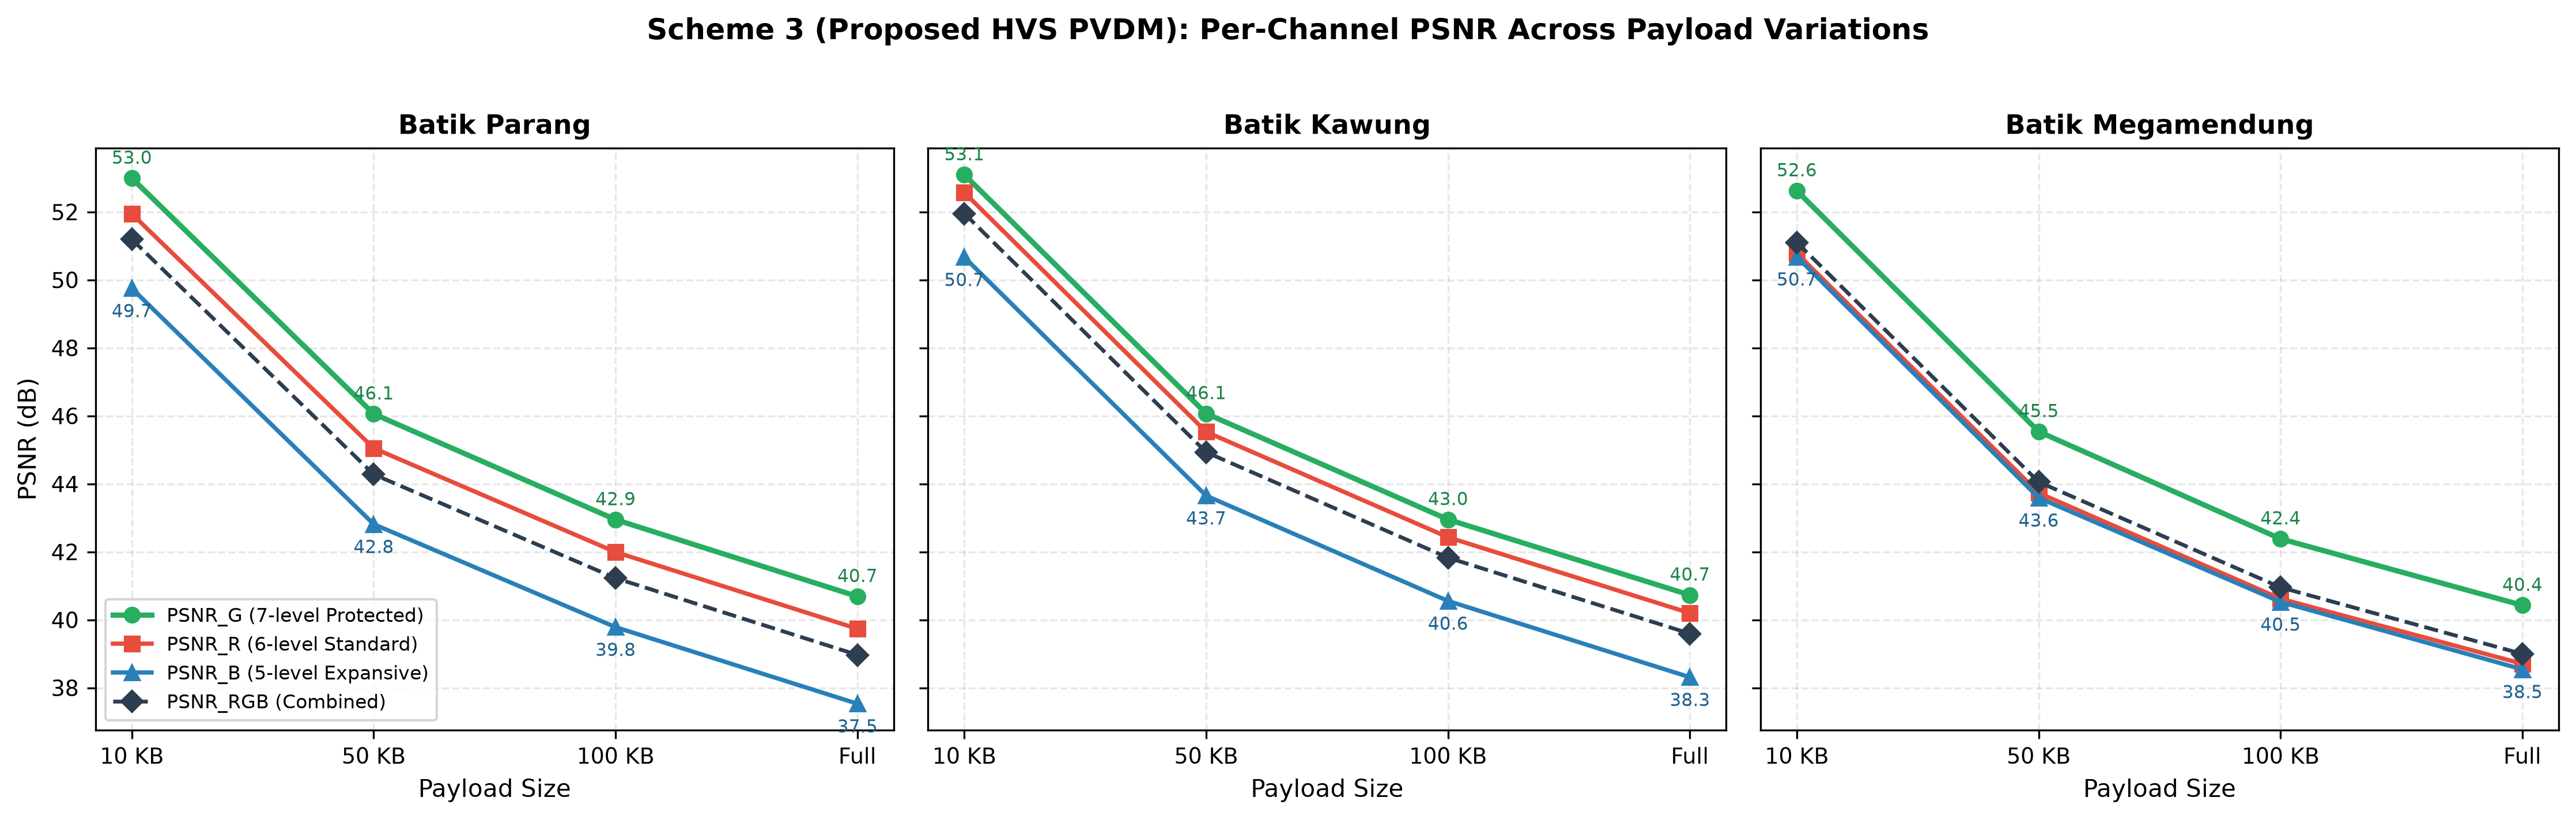
\includegraphics[width=0.95\linewidth]{figures/fig2_psnr_per_channel_vs_payload.png}
\caption{Grafik PSNR per kanal pada Skema 3 di berbagai variasi payload, membuktikan $\text{PSNR}_G$ selalu menempati posisi tertinggi di seluruh motif.}
\label{fig:psnr}
\end{figure*}

\begin{figure*}[t]
\centering
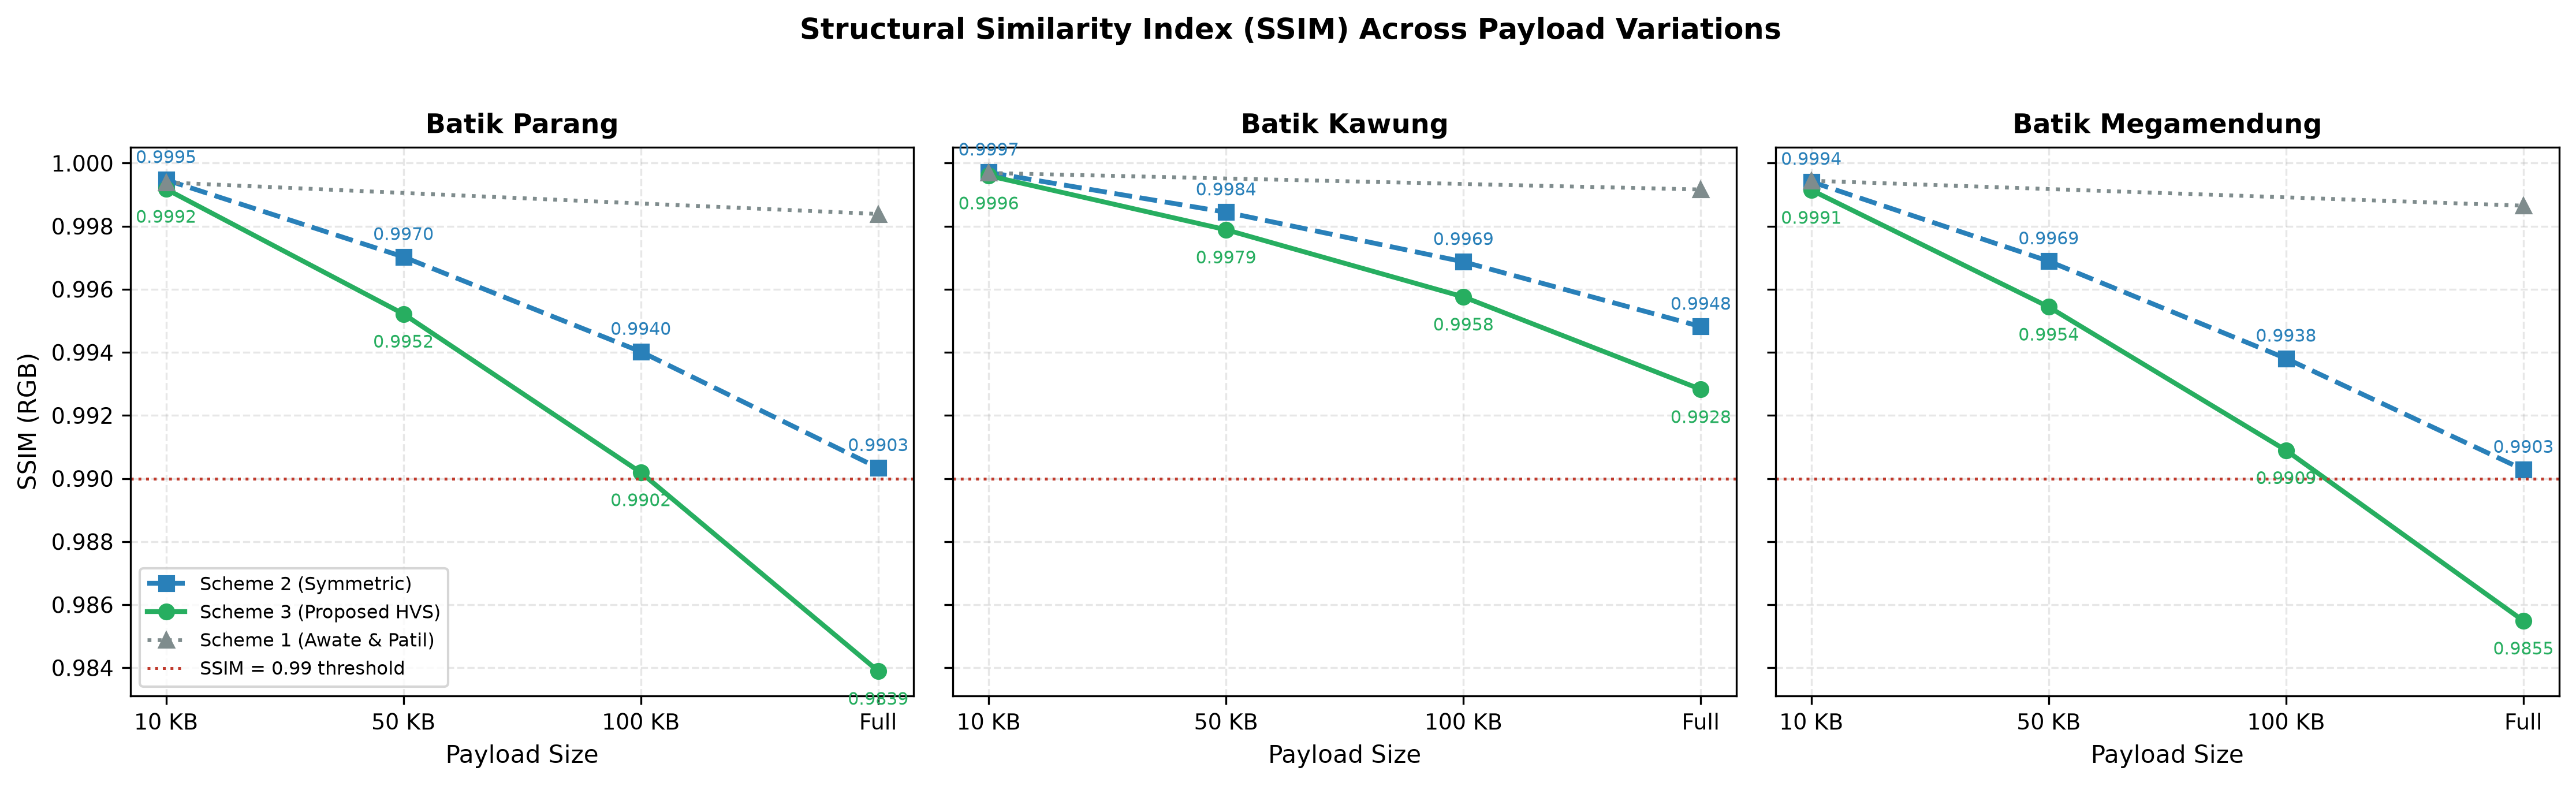
\includegraphics[width=0.95\linewidth]{figures/fig3_ssim_vs_payload.png}
\caption{Perbandingan nilai $\text{SSIM}_{\text{RGB}}$ antar skema terhadap garis ambang kualitas tinggi 0,99.}
\label{fig:ssim}
\end{figure*}

\subsection{Analisis Korelasi Tekstur Batik dan Uji Tekanan FOBP}
Tabel~\ref{tab:texture_fobp} dan Gambar~\ref{fig:texture_fobp} menguraikan hubungan kerapatan tekstur Batik terhadap kapasitas dan kejadian FOBP. Motif geometris rapat (Kawung dengan 27,65\% area tepi dan Parang 21,36\%) memberikan kapasitas lebih besar dibanding Megamendung (14,71\%), menghasilkan korelasi Pearson positif sangat kuat antara proporsi area tepi dan $\text{bpp}$ Skema~3 ($r = 0{,}9574$). Sebaliknya, korelasi area tepi terhadap FOBP lemah ($r = -0{,}1933$) karena pemicuan FOBP lebih ditentukan oleh kedekatan intensitas piksel terhadap batas 0 dan 255, seperti terlihat pada Megamendung (tepi ekstrem 0,5407\%, laju FOBP 2,65\%). Kanal Green mencatat FOBP terendah pada Parang (1.435,67) dan Kawung (798,53), dan seluruh kejadian FOBP (1,53\%--2,65\%) tertangani sempurna oleh Step~4 dengan $\text{BER} = 0{,}0\%$.

\begin{table*}[t]
\centering
\caption{Korelasi Kerapatan Tekstur Batik terhadap Kapasitas dan Kejadian FOBP pada Kapasitas Penuh ($n=15$ per Motif)}
\label{tab:texture_fobp}
\scriptsize
\setlength{\tabcolsep}{4pt}
\resizebox{\textwidth}{!}{%
\begin{tabular}{@{}lrrrrrrrrrr@{}}
\toprule
Motif & Mean $|\Delta|$ & Halus (\%) & Tepi (\%) & Ekstrem (\%) & Cap S3 (B) & BPP S3 & FOBP S1 & FOBP S2 & FOBP S3 (R/G/B) & Laju S3 \\
\midrule
Parang      & 12,25 & 78,64 & 21,36 & 0,3798 & 168.175,33 & 5,1323 & 1.197,27 & 8.846,80  & 9.822,07 (3.036/1.436/5.350)  & 2,50\% \\
Kawung      & 13,47 & 72,35 & 27,65 & 0,1208 & 171.475,13 & 5,2330 & 716,47   & 5.482,47  & 6.007,67 (2.173/799/3.037)    & 1,53\% \\
Megamendung & 9,48  & 85,29 & 14,71 & 0,5407 & 162.181,73 & 4,9494 & 383,07   & 10.929,13 & 10.406,73 (6.277/2.296/1.834) & 2,65\% \\
\bottomrule
\end{tabular}%
}
\end{table*}

\begin{figure*}[t]
\centering
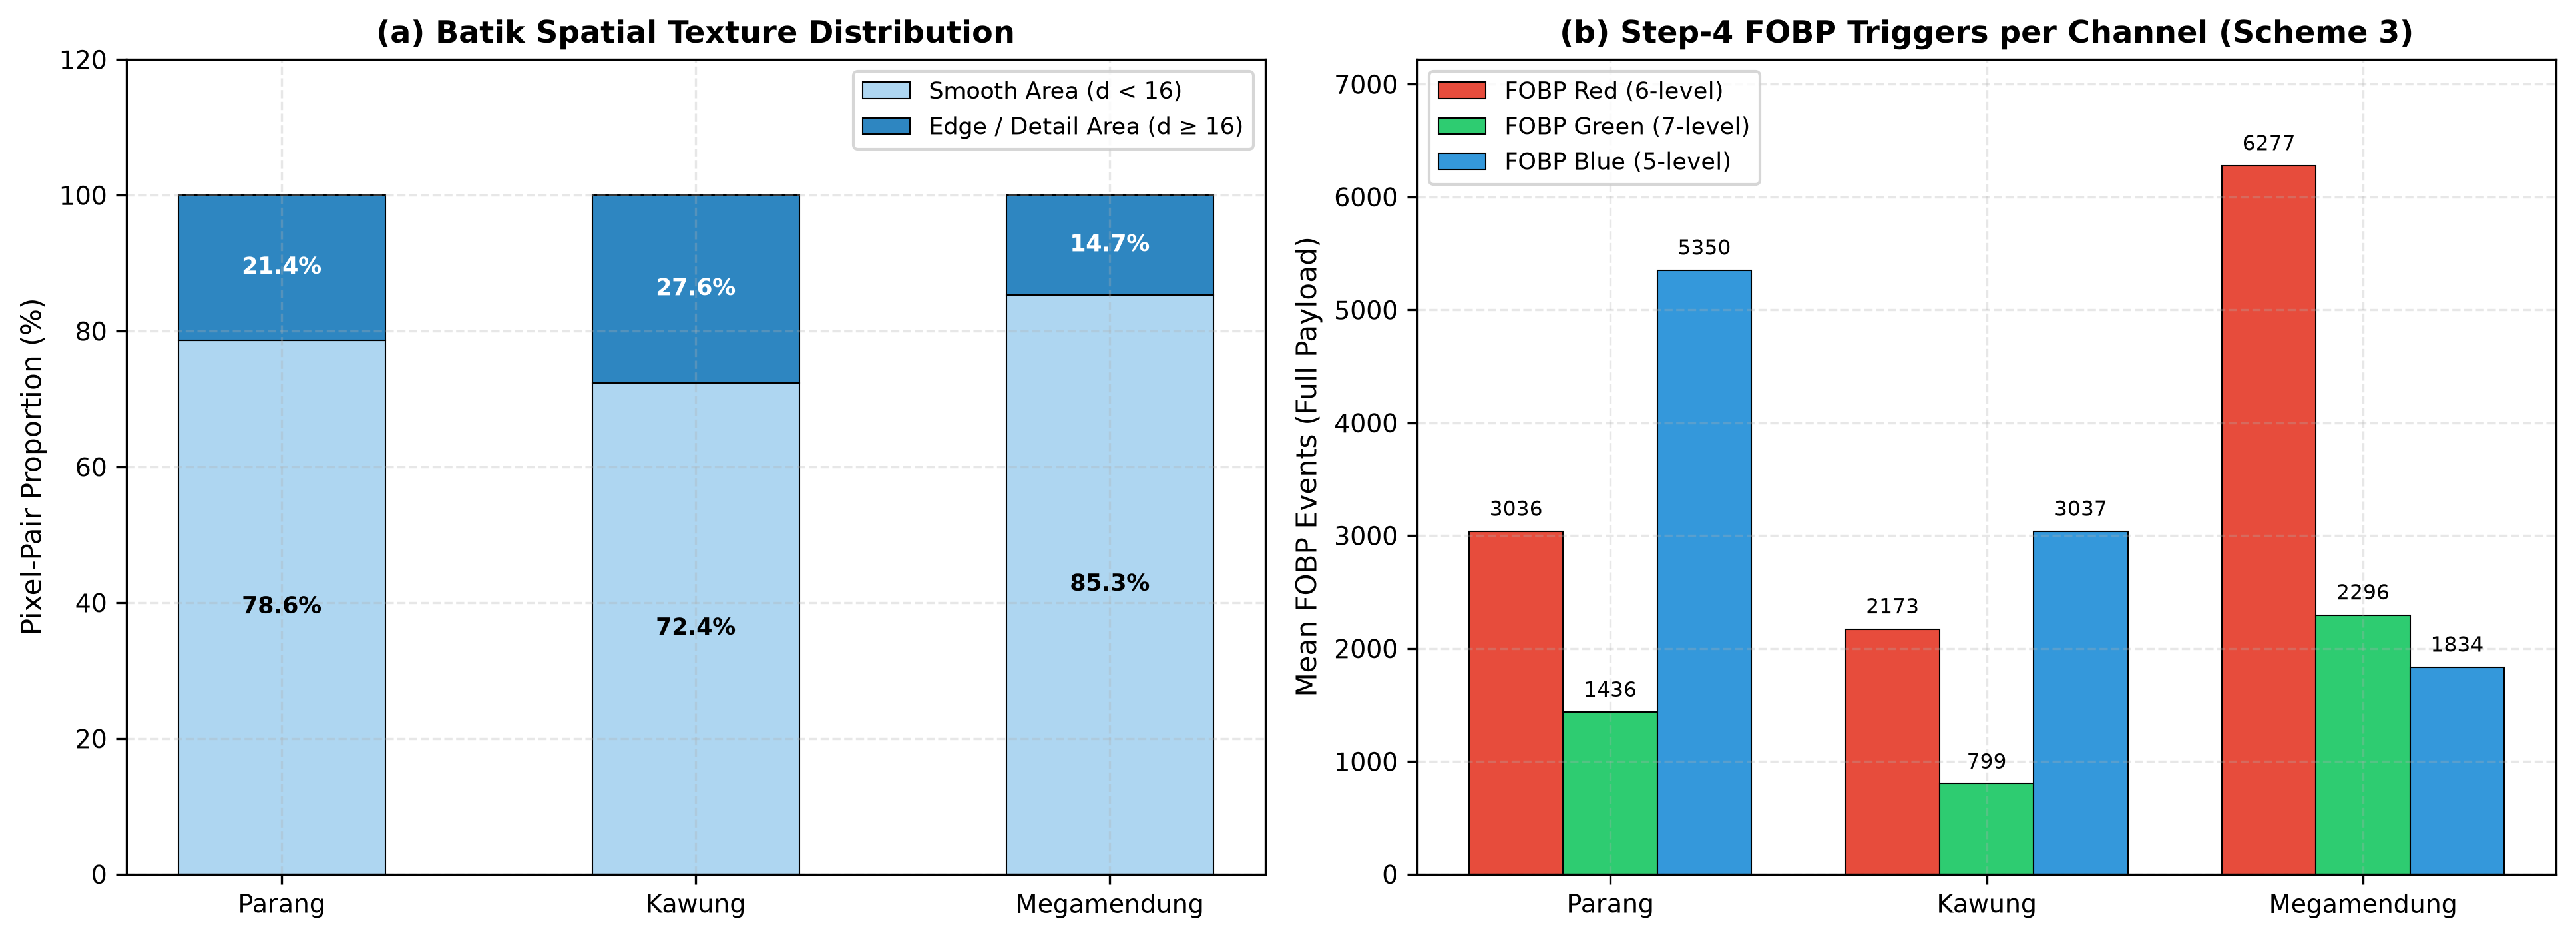
\includegraphics[width=0.92\linewidth]{figures/fig4_texture_vs_capacity_fobp.png}
\caption{Distribusi proporsi area halus vs.\ tepi pada citra Batik (a) serta frekuensi pemicuan FOBP per kanal pada Skema 3 (b).}
\label{fig:texture_fobp}
\end{figure*}

\subsection{Komparasi Visual Antar Skema dan Inspeksi Histogram RGB}
Gambar~\ref{fig:visual_schemes} menyajikan uji visual langsung antara citra asli (\textit{Cover}) dan citra stego dari Skema 1, Skema 2, serta Skema 3 pada pesan 10 KB, yaitu ukuran terbesar yang masih mampu dimuat oleh ketiga skema secara adil. Secara kasat mata tidak tampak perubahan warna maupun cacat citra pada seluruh skema, sedangkan Skema 3 selalu mencatat $\text{PSNR}_G$ paling tinggi di semua motif (53,53 dB pada Parang, 51,93 dB pada Kawung, dan 55,31 dB pada Megamendung). Selanjutnya, Gambar~\ref{fig:visual_hist} memuat perbandingan \textit{Cover} dan \textit{Stego} Skema 3 pada pesan 50 KB beserta kurva histogram RGB; grafik histogram citra stego tampak berimpit rapat dengan citra asli tanpa pergeseran warna.

\begin{figure*}[t]
\centering
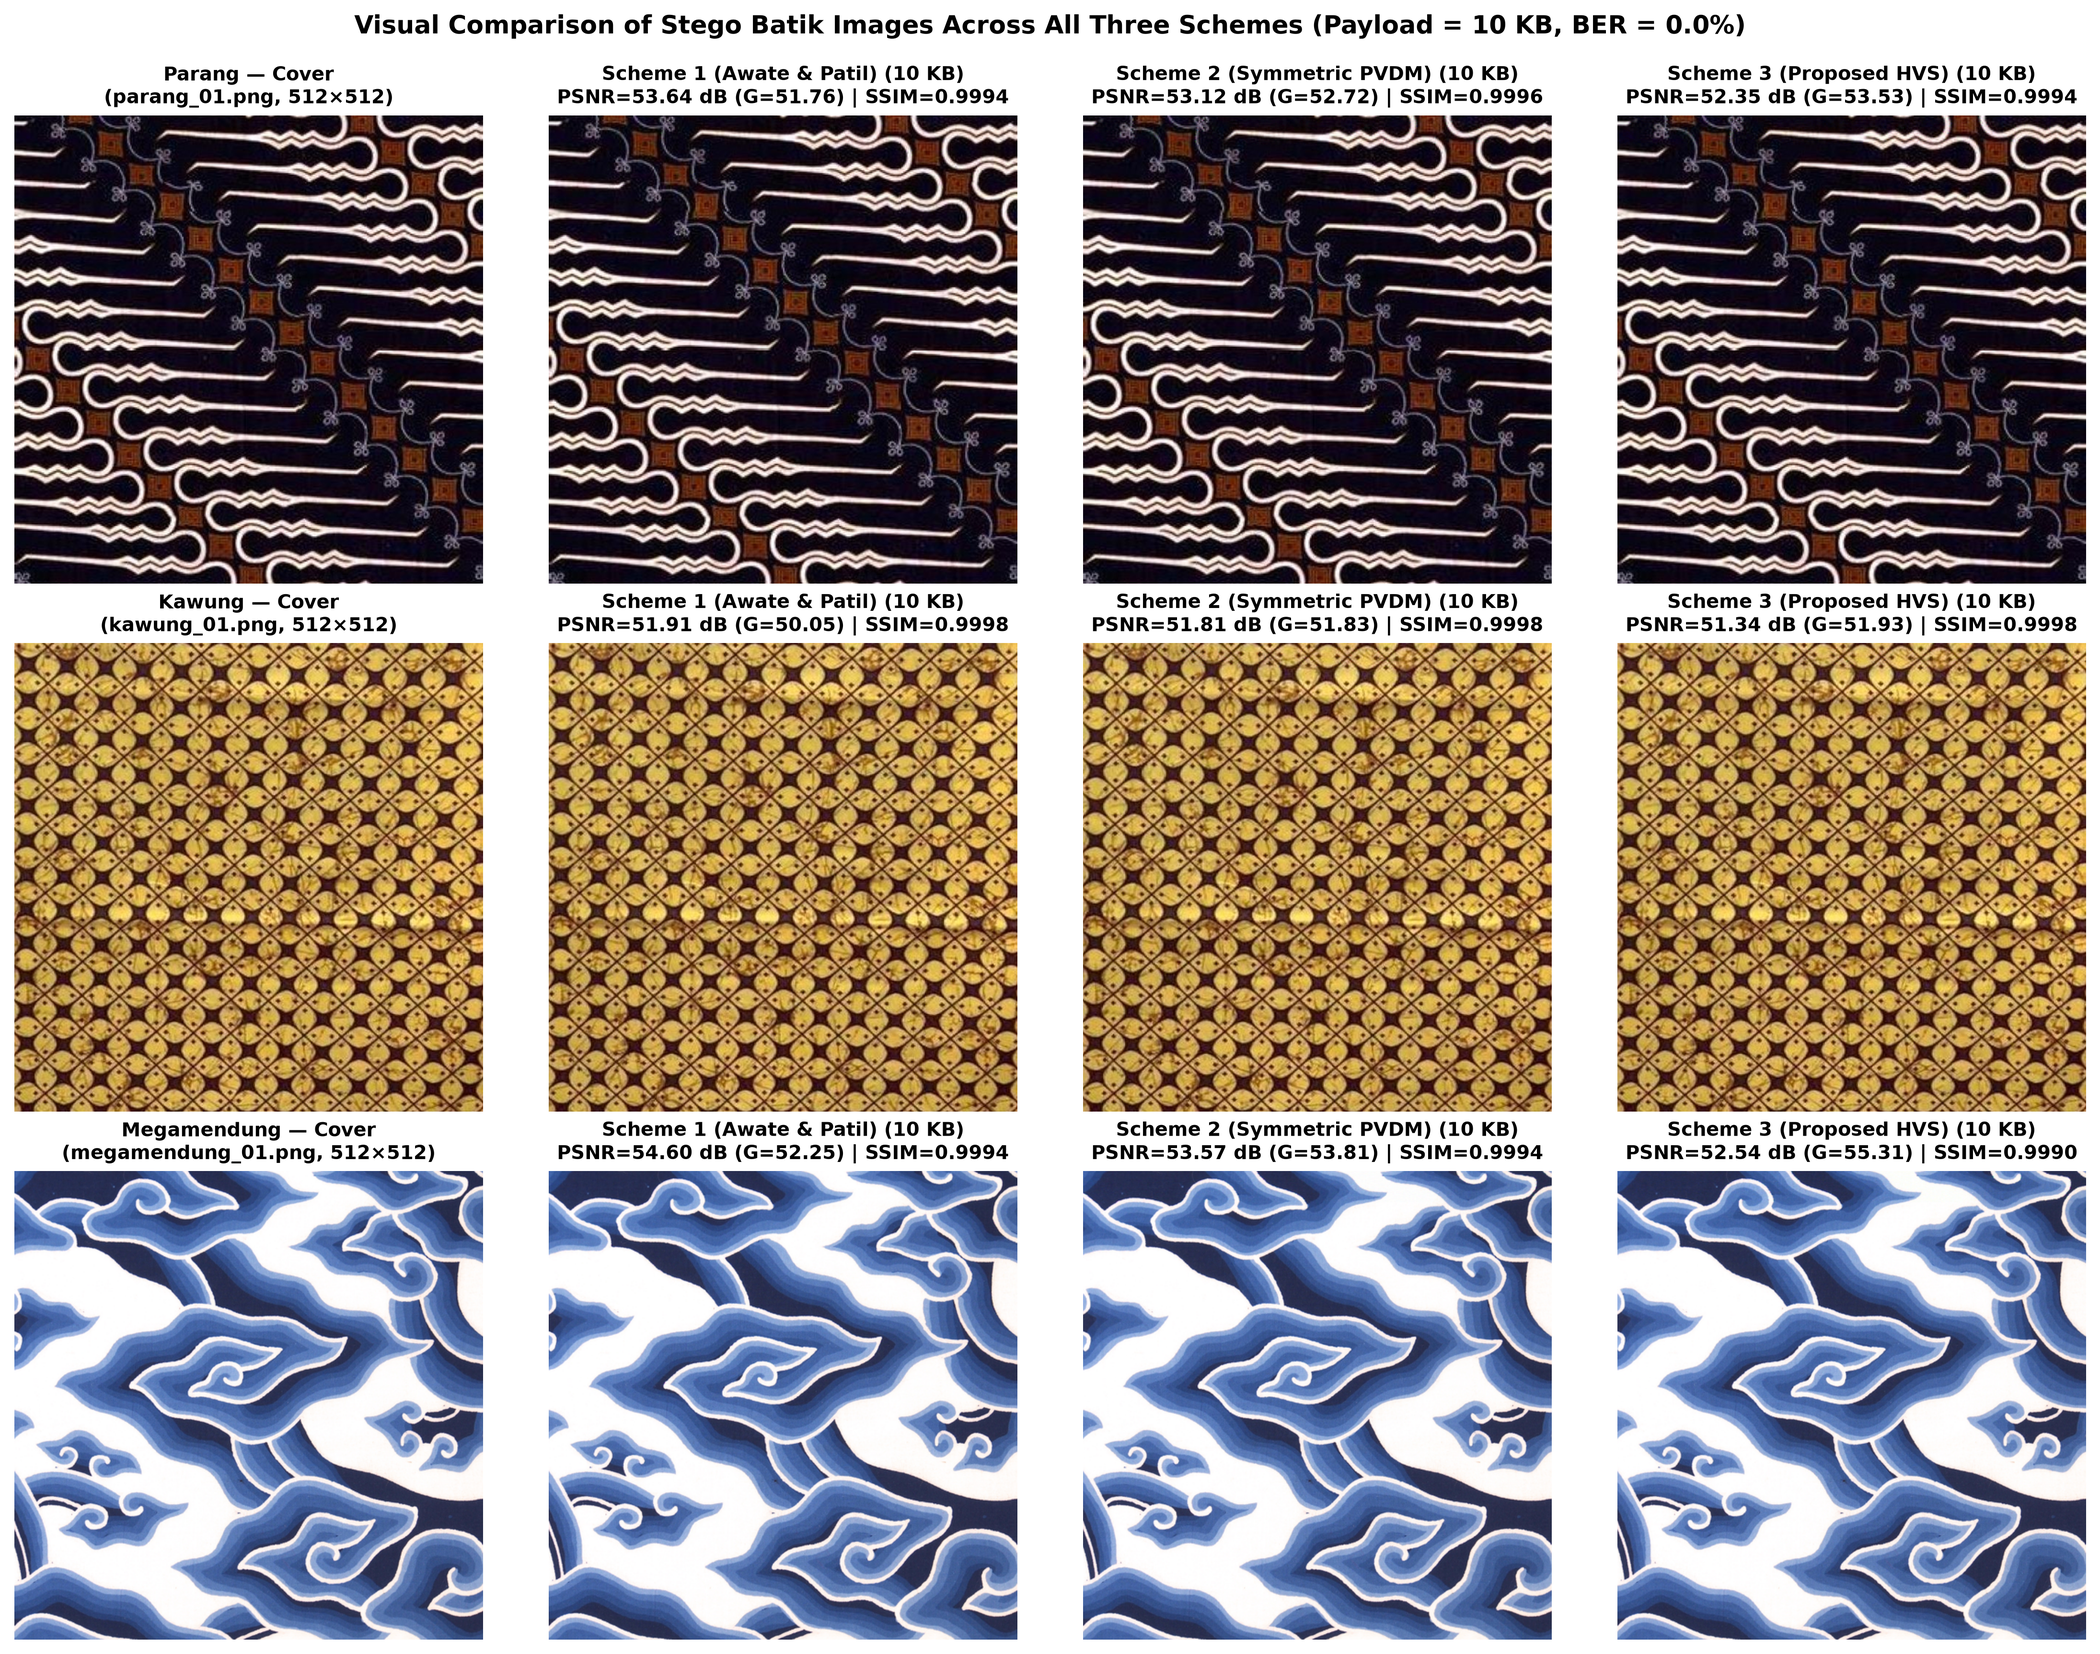
\includegraphics[width=0.95\linewidth]{figures/fig7_schemes_visual_comparison_10kb.png}
\caption{Komparasi visual berdampingan antara citra Cover, Skema 1, Skema 2, dan Skema 3 pada payload seragam 10 KB ($\text{BER} = 0{,}0\%$).}
\label{fig:visual_schemes}
\end{figure*}

\begin{figure*}[t]
\centering
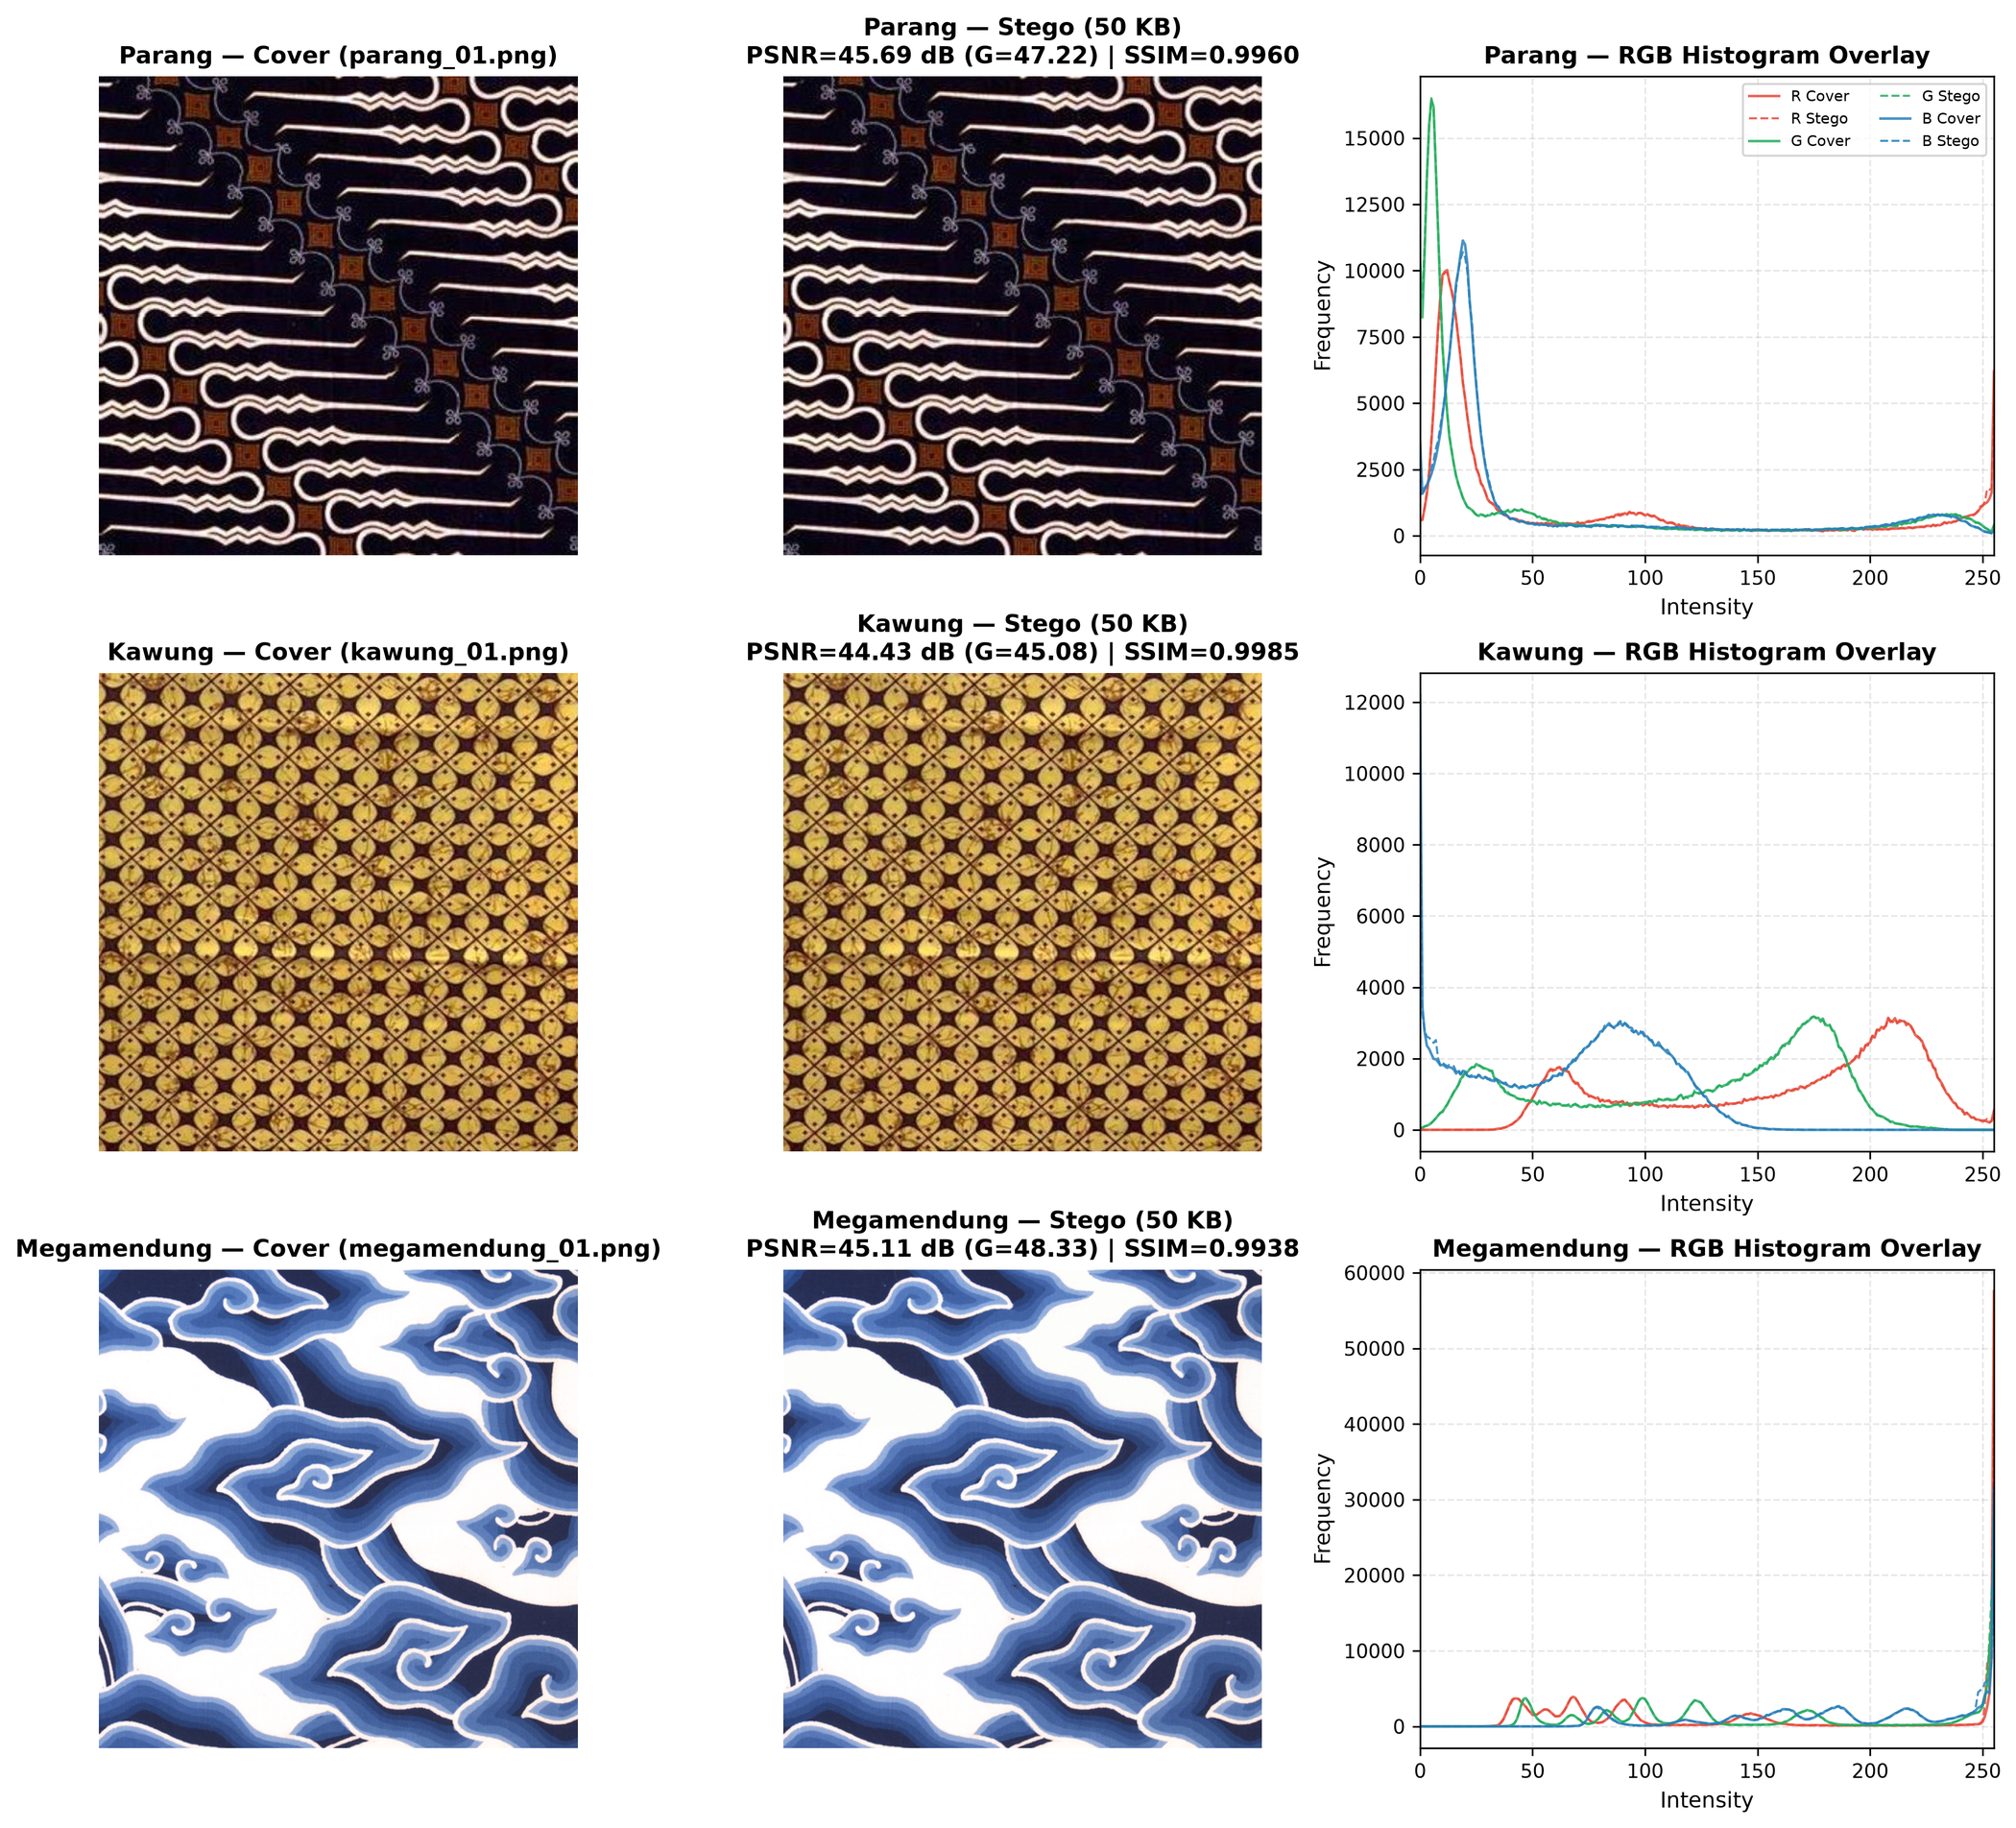
\includegraphics[width=0.90\linewidth]{figures/fig6_combined_visual_comparison.png}
\caption{Perbandingan visual Cover vs.\ Stego Skema 3 (payload 50 KB) dan tumpang tindih histogram RGB pada Parang, Kawung, dan Megamendung.}
\label{fig:visual_hist}
\end{figure*}

\FloatBarrier

\section{Kesimpulan}

Penelitian ini merancang dan mengevaluasi metode steganografi PVDM RGB dengan tabel rentang kuantisasi asimetris berbasis HVS secara terkontrol (\textit{Batik vs.\ Batik}) pada 45 citra Batik Nusantara. Dengan memproteksi kanal Green (7-level), mempertahankan kanal Red (6-level), dan mengekspansi kanal Blue (5-level) secara simultan, Skema~3 meningkatkan kapasitas penyisipan sebesar +519,29\% hingga +566,33\% dibandingkan \textit{Modified Pixel Indicator} Awate dan Patil (Skema~1) serta +1,34\% hingga +2,09\% dibandingkan PVDM RGB Simetris (Skema~2). Hasil pengujian mengonfirmasi bahwa $\text{PSNR}_G$ selalu tertinggi di seluruh motif dan variasi pesan (40,43--53,09~dB), $\text{SSIM}_Y$ mengungguli Skema~2 hingga kapasitas penuh (0,9969--0,9981), $\text{SSIM}_{\text{RGB}} > 0{,}99$ terjaga hingga 100~KB, kerapatan tepi Batik berkorelasi sangat kuat terhadap kapasitas ($r = 0{,}9574$), dan ekstraksi buta mencapai 100\% \textit{lossless} ($\text{BER} = 0{,}0\%$). Penelitian lanjutan dapat diarahkan pada pengujian ketahanan terhadap kompresi \textit{lossy} (JPEG) serta serangan steganalisis statistik seperti \textit{RS analysis} dan \textit{pixel-difference histogram} (PDH).

\bibliographystyle{IEEEtran}
\bibliography{refs}

\end{document}
